%generare il pdf con il comando: pdflatex main.tex
\documentclass[a4paper, oneside, openany,dvipsnames,table]{article}
\usepackage{../template/sos}
\usepackage{eurosym}
\usepackage{amssymb}% http://ctan.org/pkg/amssymb
\usepackage{pifont}% http://ctan.org/pkg/pifont
\usepackage{listings}
\definecolor{bluSOS}{RGB}{48, 84, 150}
\newcommand{\shellcmd}[1]{\\\indent\indent\texttt{\footnotesize\$ #1}\\}
%\WithSuffix\def\shellcmd*#1{\indent\indent\texttt{\footnotesize\$ #1}\\}
\newcommand{\Titolo}{Piano di Progetto}

\newcommand{\Gruppo}{Sons Of SWE}

\newcommand{\Redazione}{Panozzo Stefano \newline Favero Andrea \newline Dalla Riva Giovanni \newline Federico Caldart \newline Eleonora Thiella}

\newcommand{\ACapoRedazione}{Panozzo Stefano \newline Favero Andrea \newline Dalla Riva Giovanni \newline Federico Caldart \newline Eleonora Thiella}

\newcommand{\Verifica}{Dalla Riva Giovanni \newline Menegon Lorenzo \newline Cavallin Giovanni \newline Panozzo Stefano}

\newcommand{\Approvazione}{Cavallin Giovanni \newline Favero Andrea \newline Caldart Federico}

\newcommand{\Distribuzione}{Vardanega Tullio\newline Cardin Riccardo \newline Gruppo Sons Of SWE}

\newcommand{\Uso}{Esterno}


\newcommand{\Data}{07 Maggio 2018}

\newcommand{\NomeProgetto}{Progetto Marvin}

\newcommand{\Mail}{sonsofswe.swe@gmail.com}


\newcommand{\DescrizioneDoc}{Documento contenente il piano di progetto relativo al \NomeProgetto{} scelto dal gruppo \Gruppo.}

\newcommand{\versione}{3.0.0}




\begin{document}
%\copertina{}

	\begin{titlepage}
		\begin{center}

			\begin{center}
				%sostituire con immagine copertina del gruppo
				\centerline{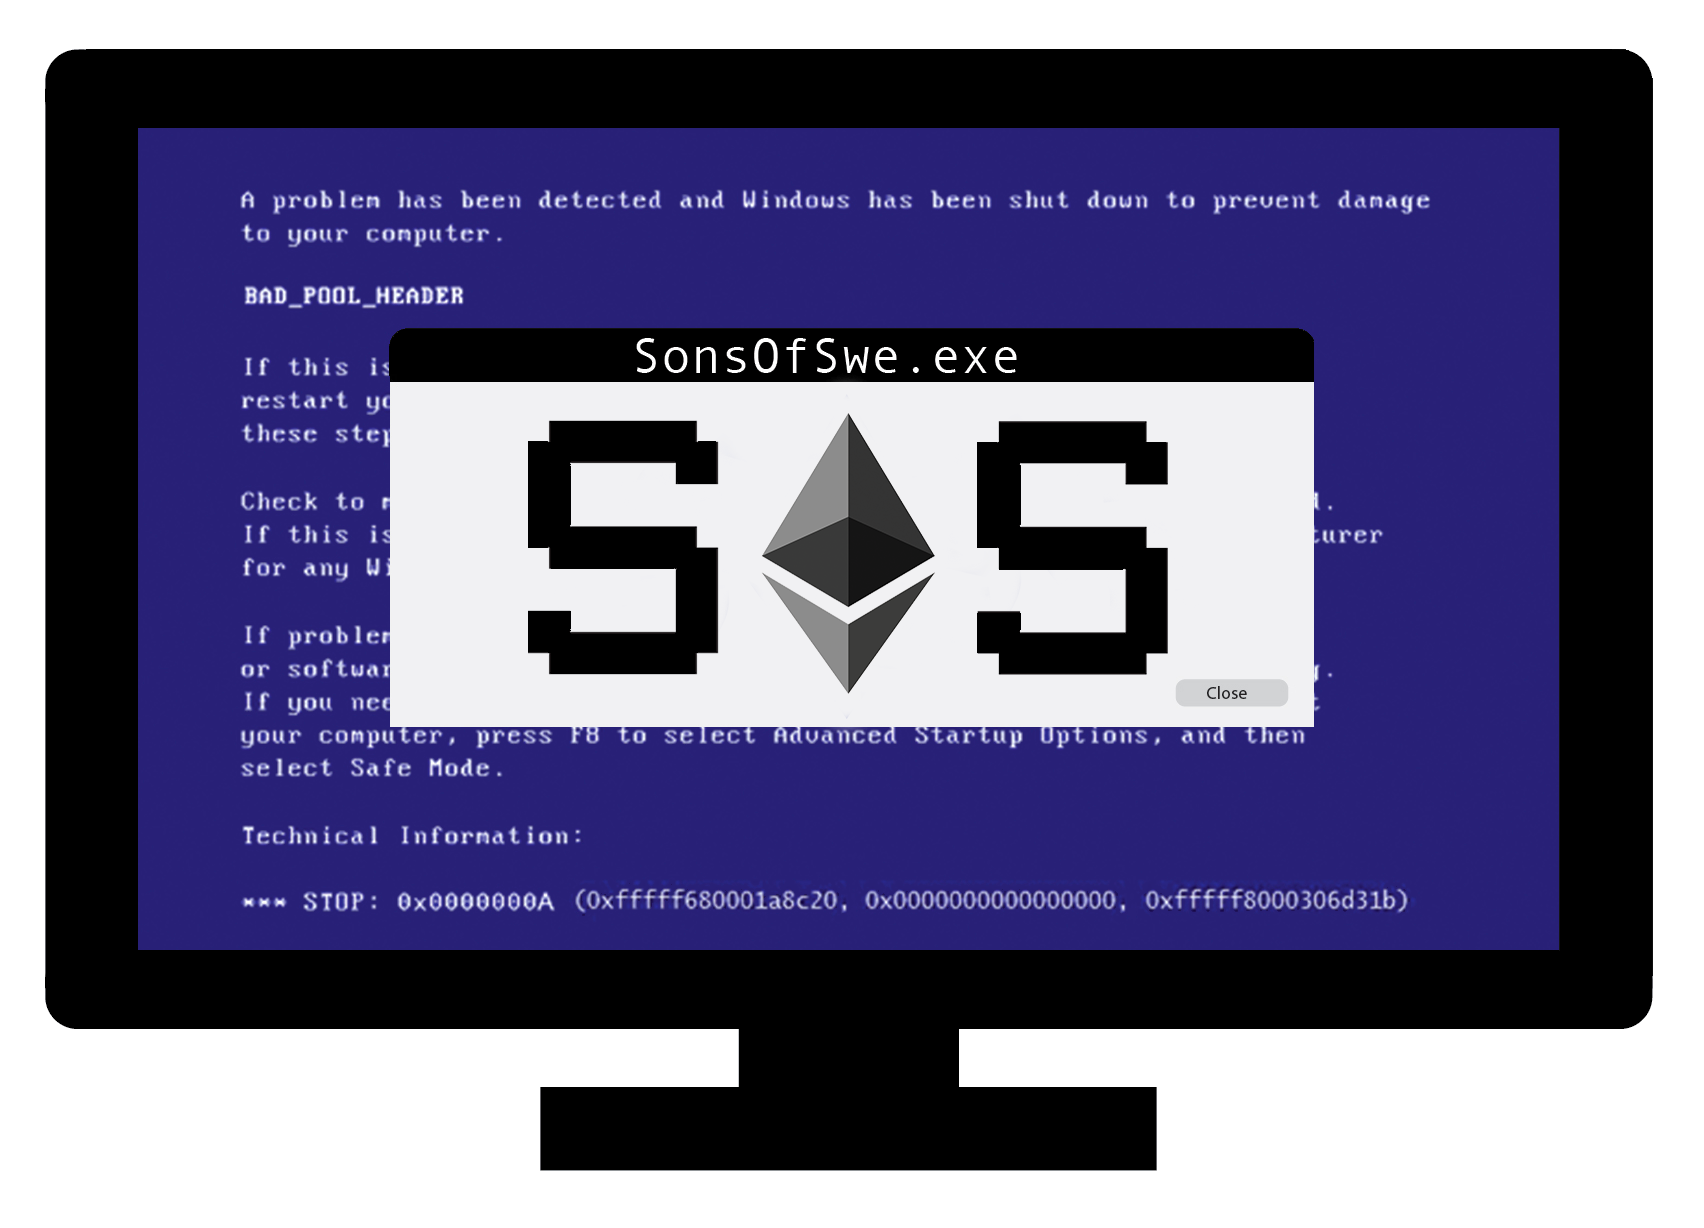
\includegraphics[scale=0.20]{../template/img/logo.png}}
			\end{center}

			\vspace{1cm}

			\begin{Huge}
				\textbf{\Titolo{}} \\
			\end{Huge}

			\vspace{9pt}

			\begin{large}
				\textbf{\Gruppo{}}\ - \textbf{\NomeProgetto{}}\\%\Data{}
				\vspace{6pt}
				\Mail{}
			\end{large}

			\vspace{15pt}

			\bgroup
			\def\arraystretch{1.3}
			\centering
			\begin{tabular}{r|L{5cm}}
				\multicolumn{2}{c}{\textbf{Informazioni sul documento} } \\ \hline
				\textbf{Uso} & \Uso \\
				\textbf{Distribuzione} & \Distribuzione{}
			\end{tabular}
			\egroup

			\vspace*{\fill}

			\begin{center}
				\textbf{Descrizione\\}
				\DescrizioneDoc{}
			\end{center}

		\end{center}
	\end{titlepage}


%%%%%%%%%%%%%%%%%%%%%%%%%%%%%%%%%%%%%%%%%%%%%%%%%%%%%%%%%%%%%%%%%%%%%%%%%%%%%%%%%%%%%%%%%%%%%%%%%%%%%%%
%SOMMARIO
\newpage
\tableofcontents
\newpage
\listoffigures
\newpage
%%%%%%%%%%%%%%%%%%%%%%%%%%%%%%%%%%%%%%%%%%%%%%%%%%%%%%%%%%%%%%%%%%%%%%%%%%%%%%%%%%%%%%%%%%%%%%%%%%%%%%%
%PARAGRAFI
\hypersetup{linkcolor=bluSOS}
\section{Introduzione}
\subsection{Scopo del documento}
Questo documento ha lo scopo di descrivere gli \emph{attori}\ped{G} del sistema, individuare i \emph{casi d'uso}\ped{G} a partire dai \emph{requisiti}\ped{G} e fornire una visione chiara ai \progs{} sul problema da trattare. I requisiti verranno classificati in questo documento a seguito di una trattazione col proponente.

\subsection{Scopo del prodotto}
Lo scopo del prodotto è quello di realizzare un \emph{prototipo}\ped{G} di \emph{Uniweb}\ped{G} come \emph{ÐApp}\ped{G} in esecuzione su \emph{Ethereum}\ped{G}. I cinque attori principali che si rapportano con Marvin sono:
\begin{itemize}
	\item Utente non autenticato;
	\item Università;
	\item Amministratore;
	\item Professori;
	\item Studenti.
\end{itemize} 
Il portale deve quindi permettere agli studenti di accedere alle informazioni riguardanti le loro carriere universitarie, di iscriversi agli esami, di accettare o rifiutare voti e di poter vedere il loro libretto universitario.
Ai professori deve invece essere permesso di registrare i voti degli studenti.
L'università ogni anno crea una serie di corsi di laurea rivolti a studenti, dove ognuno di essi comprende un elenco di esami disponibili per anno accademico. Ogni esame ha un argomento, un numero di crediti e un professore associato. Gli studenti si iscrivono ad un corso di laurea e tramite il libretto elettronico mantengono traccia ufficiale del progresso.

\subsection{Glossario}
Nel documento Glossario i termini tecnici, gli acronimi e le abbreviazioni sono definiti in modo chiaro e conciso, in modo tale da evitare ambiguità e massimizzare la comprensione dei documenti.
\newline I vocaboli presenti in esso saranno posti in corsivo e presenteranno una "G" maiuscola a pedice.
\subsection{Riferimenti}
\subsubsection{Normativi}
\begin{itemize}
	\item \textcolor{red}\NdP
\end{itemize}

\subsubsection{Informativi}
\begin{itemize}
	\item Capitolato d'appalto C6: Marvin. Reperibile all'indirizzo:\\ 
	\href{http://www.math.unipd.it/~tullio/IS-1/2017/Progetto/C6.pdf}{http://www.math.unipd.it/~tullio/IS-1/2017/Progetto/C6.pdf};
	\item \textcolor{red}\SdF;
\end{itemize}

\section{Descrizione generale}
	\subsection{Contesto d'uso del prodotto}
	Il prodotto finale vuole essere una sorta di \emph{PoC}\ped{G} per dimostrare la fattibilità di utilizzo di tali tecnologie in quest’ambito. L’applicazione sarà un prototipo di Uniweb, quindi si colloca in un contesto universitario dove gli attori si approcciano al sistema come nell’attuale Uniweb. La differenza sta nel \emph{back-end}\ped{G} dove, invece del classico sistema \emph{client}\ped{G}/\emph{server}\ped{G}, troviamo un database distribuito che sfrutta la piattaforma Ethereum.
	
	\subsection{Caratteristiche degli utenti}
	Questo prodotto deve risultare accessibile ad un'ampia categoria di utenti senza particolari competenze. L’interfaccia dovrà quindi essere il più chiara ed intuitiva possibile. Verrà fornito anche un \MU{} con tutte le indicazioni necessarie per consentire il corretto utilizzo del prodotto.
	
	\subsection{Assunzione dipendenze}
	Per il corretto funzionamento dell’applicazione sarà necessario l’utilizzo di un browser che sia compatibile con \emph{HTML5}\ped{G}, \emph{SCSS}\ped{G} e \emph{Javascript}\ped{G}.

\pagebreak
%%%%%%%%%%%%%%%%%%%%%%%%%%%%%%%%%%%%%%%%%%%%%%%%%%%%%%%%%%%%%%%%%%%%%%%%%%%%%%%%%%%%%%%%%%%%%%%%%%%%%%%
\section{Requisiti di sistema}
Per l'installazione e l'utilizzo di questo software sono richiesti alcuni prerequisiti:
\begin{itemize}
	\item Browser web Google Chrome (aggiornato alla versione 60 o superiori) o Mozilla Firefox (aggiornato alla versione 50 o superiori);
	\item Plugin Metamask (aggiornato alla versione 4.7.1 o superiori) per i browser di cui sopra; \\
	\url{https://metamask.io/}
	\item Git \\
	\url{https://git-scm.com/downloads}
	\item Python aggiornato alla versione 2.7; \\
	\url{https://www.python.org/downloads/}
	\item Node package manager alla versione 6, e Node alla 8.11.2 \\
	\url{https://nodejs.org/it/}
	\item Nel caso si utilizzi Windows sarà necessario installare \textit{windows-build-tools} digitando nella powershell: 
	\begin{lstlisting}
		npm install --global --production windows-build-tools
	\end{lstlisting}

	 
\end{itemize}
\pagebreak
\section{Installazione ed esecuzione}
Il codice relativo alla Product Baseline lo si può trovare al seguente link:
\begin{center}
	\url{linkAllaRepo}
\end{center}
Una volta fatto il clone della repository o dopo aver scaricato lo zip, sono necessari i seguenti passi per far partire l'applicazione:
\begin{enumerate}
	\item Posizionarsi nella root della repo ed eseguire nella shell:
		\begin{lstlisting}
	npm install -g ganache-cli
	npm install -g truffle
	npm i
		\end{lstlisting}
	\item In seguito sempre nella shell:
		\begin{lstlisting}
	./startBlockchain.ps1
		\end{lstlisting}
	\item Infine è necessario eseguire:
		\begin{lstlisting}
	./loadProject.ps1
		\end{lstlisting}
\end{enumerate}

A questo punto noterai che il tuo browser predefinito ha aperto automaticamente l'homepage.
Ora dovrai connetteri a Metamask: nel tuo browser clicca sull'icona di Metamask e accetta l'informativa sulla privacy e le condizioni d'uso. Poi clicca su \textbf{Main Network} e scegli \textbf{Custom RPC}, inserisci nel primo form \textbf{http://localhost:9545} come in Figura~\ref{fig:metamask1} e clicca su  \textbf{Save}.
%Now you have to connect MetaMask: in your browser click on the MetaMask icon and accept the Privacy Notice and the Terms of use. Then click on \textbf{Main Network} and choose \textbf{Custom RPC}, type in the first form \textbf{http://localhost:9545} as in Figure~\ref{fig:metamask1} and click \textbf{Save}.

\begin{figure}[h]
\centering
\includegraphics[height=3in]{./img/settings.png}
\caption{Setta l'RPC inserendo \textbf{http://localhost:9545}}
\label{fig:metamask1}
\end{figure}

Ora, come in Figura~\ref{fig:metamask2}, clicca su \textbf{Import Existing DEN} e (vedi Figura~\ref{fig:metamask3}) inserisci la frase \textbf{candy maple cake sugar pudding cream honey rich smooth crumble sweet treat} e la password che vuoi usare per il tuo account.


\begin{figure}[h]
\centering
\includegraphics[height=1.8in]{./img/importa.png}
\caption{Clicca su \textbf{Import Existing DEN}}
\label{fig:metamask2}
\end{figure}

\begin{figure}[h]
\centering
\includegraphics[height=3in]{./img/stringa_psw.png}
\caption{Inserisci la seed phrase e la password che vuoi usare}
\label{fig:metamask3}
\end{figure}
	

\pagebreak
\section{Requisiti soddisfatti}
\subsection{Tabella del soddisfacimento dei requisiti}
\begin{table}[hp]
\centering
\begin{tabular}{|c|c|c|}
\hline
ID requisito & Soddisfacimento nell'architettura & Soddisfacimento nel codice \\ \hline
R0F1         & SODDISFATTO                       & SODDISFATTO                \\ \hline
R0F2         & SODDISFATTO                       & SODDISFATTO                \\ \hline
R0F3         & SODDISFATTO                       & SODDISFATTO                \\ \hline
R0F4        & SODDISFATTO                       & SODDISFATTO                \\ \hline
R0F5        & SODDISFATTO                       & SODDISFATTO                \\ \hline
R0F6        & SODDISFATTO                       & SODDISFATTO                \\ \hline
R2F7        & SODDISFATTO                       & NON SODDISFATTO                \\ \hline
R2F8        & SODDISFATTO                       & NON SODDISFATTO                \\ \hline
R2F9        & SODDISFATTO                       & NON SODDISFATTO                \\ \hline
R2F10        & SODDISFATTO                       & NON SODDISFATTO                \\ \hline
R2F11        & SODDISFATTO                       & NON SODDISFATTO                \\ \hline
R2F13        & SODDISFATTO                       & NON SODDISFATTO                \\ \hline
R2F14        & SODDISFATTO                       & NON SODDISFATTO                \\ \hline
R0F15        & SODDISFATTO                       & SODDISFATTO                \\ \hline
R0F16        & SODDISFATTO                       & SODDISFATTO                \\ \hline
R0F17        & SODDISFATTO                       & SODDISFATTO                \\ \hline
R0F18        & SODDISFATTO                       & SODDISFATTO                \\ \hline
R0F19        & SODDISFATTO                       & NON SODDISFATTO                \\ \hline
R2F20        & SODDISFATTO                       & NON SODDISFATTO                \\ \hline
R2F21        & SODDISFATTO                       & NON SODDISFATTO                \\ \hline
R2F22        & SODDISFATTO                       & NON SODDISFATTO                \\ \hline
R0F23        & SODDISFATTO                       & SODDISFATTO                \\ \hline
R0F24        & SODDISFATTO                       & SODDISFATTO                \\ \hline
R2F25        & SODDISFATTO                       & NON SODDISFATTO                \\ \hline
R0F26        & SODDISFATTO                       & SODDISFATTO                \\ 
\hline
\end{tabular}
\caption{Requisiti soddisfatti}
\end{table}
\clearpage

\subsection{Grafici sui requisiti soddisfatti}
\begin{figure}[hp]
\centering
\includegraphics[height=7cm]{img/RequisitiSoddisfatti.png}\\
\caption{Requisiti soddisfatti}
\end{figure}

\begin{figure}[hp]
\centering
\includegraphics[height=7cm]{img/RequisitiObbligatoriSoddisfatti.png}\\
\caption{Requisiti obbligatori soddisfatti}
\end{figure}

\pagebreak
\section{Casi d'uso soddisfatti}
\subsection{Tabella del soddisfacimento dei casi d'uso}
\begin{table}[hp]
\centering
\begin{tabular}{|c|c|c|}
\hline
ID caso d'uso & Soddisfacimento nell'architettura & Soddisfacimento nel codice \\ \hline
UC1         & SODDISFATTO                       & NON SODDISFATTO                \\ \hline
UC2         & SODDISFATTO                       & NON SODDISFATTO                \\ \hline
UC3         & SODDISFATTO                       & NON SODDISFATTO                \\ \hline
UC4         & SODDISFATTO                       & NON SODDISFATTO                \\ \hline
UC6         & SODDISFATTO                       & SODDISFATTO                \\ \hline
UC7         & SODDISFATTO                       & SODDISFATTO                \\ \hline
UC8         & SODDISFATTO                       & SODDISFATTO                \\ \hline
UC9         & SODDISFATTO                       & SODDISFATTO                \\ \hline
UC10         & SODDISFATTO                       & SODDISFATTO                \\ \hline
UC11         & SODDISFATTO                       & NON SODDISFATTO                \\ \hline
UC12         & SODDISFATTO                       & NON SODDISFATTO                \\ \hline
UC13         & SODDISFATTO                       & NON SODDISFATTO                \\ \hline
UC14         & SODDISFATTO                       & NON SODDISFATTO                \\ \hline
UC15         & SODDISFATTO                       & NON SODDISFATTO                \\ \hline
UC16         & SODDISFATTO                       & NON SODDISFATTO                \\ \hline
UC17         & SODDISFATTO                       & NON SODDISFATTO                \\ \hline
UC18         & SODDISFATTO                       & NON SODDISFATTO                \\ \hline
UC19         & SODDISFATTO                       & NON SODDISFATTO                \\ \hline
UC20         & SODDISFATTO                       & NON SODDISFATTO                \\ \hline
UC21         & SODDISFATTO                       & NON SODDISFATTO                \\ \hline
UC22         & SODDISFATTO                       & NON SODDISFATTO                \\ \hline
UC23         & SODDISFATTO                       & SODDISFATTO                \\ \hline
UC24         & SODDISFATTO                       & NON SODDISFATTO                \\ \hline
UC25         & SODDISFATTO                       & NON SODDISFATTO                \\ \hline
UC26         & SODDISFATTO                       & NON SODDISFATTO                \\ \hline
UC27         & SODDISFATTO                       & SODDISFATTO                \\ \hline
UC28         & SODDISFATTO                       & SODDISFATTO                \\ \hline
UC29         & SODDISFATTO                       & NON SODDISFATTO                \\ \hline
UC30         & SODDISFATTO                       & SODDISFATTO                \\ \hline
UC31         & SODDISFATTO                       & SODDISFATTO                \\ \hline
UC32         & SODDISFATTO                       & SODDISFATTO                \\ \hline
UC33         & SODDISFATTO                       & SODDISFATTO                \\ \hline

\end{tabular}
\caption{Casi d'uso soddisfatti}
\end{table}
\clearpage

\subsection{Grafici sui casi d'uso soddisfatti}
\begin{figure}[hp]
\centering
\includegraphics[height=7cm]{img/UCSoddisfatti.png}\\
\caption{Casi d'uso soddisfatti}
\end{figure}





\end{document}


